\chapter{Model presentation}
\label{chap:Model Presentation}


\section{Ecological bases}

This model has been inspired by earlier works carried out by \href{https://gdri-ehede.univ-fcomte.fr}{GDRI EHEDE} researchers \citep{Li2015,Clauzel2015,Li2017}.

In brief, after \citet{Li2015}, the black-and-white snub-nosed monkey \textit{Rhinopithecus bieti} is endemic to Yunnan and Tibet, China, and categorized as "endangered" in the IUCN Red List. Surveys have shown that the monkeys live in 15 isolated groups, 12 of them in Yunnan, in a narrow range of the Three Parallel Rivers region, one of the most ecologically important areas of China, the rugged terrain of which makes it difficult to carry out surveys. The species is threatened by habitat alteration, poaching and economic activities such as farming and collection of timber. The areas between populations are damaged by logging, grazing, mining, agriculture and firewood collection. Because of this habitat fragmentation the monkeys may incur a high energy cost if they travel long distances between habitat patches. Fragmentation may subsequently prevent genetic exchange between populations, making the species more vulnerable to extinction. Where required, reserve managers need to establish habitat corridors to facilitate exchange between populations, identifying priority areas for restoration to increase landscape connectivity.

"Snubbies" is a nickname given to the species.

\section{Geography and data}

 Tab.~\ref{tab:habitats} describes the 5 habitat types defined by \citet{Li2017} and fig.~\ref{fig:studyarea} shows the study area and the location of the monkey groups with their ID number.
 
 The shapefile \texttt{source2P} corresponds to this map, and the predefined style file \texttt{source2P.qml} can be used in QGIS for a better display.
 
 The shapefile \texttt{groups} gives the geographical limit of each monkey group. The group ID number, the name of the area and a population size estimate are given as attributes.

 \begin{table}[ht]
 	\centering
 	\caption{Habitat quality and composition after \citet{Li2017}}
 	\label{tab:habitats}
 	\begin{tabular}{lllcc}
 		\hline
 		ID & habitat type & Land cover & Altitude & Cost value \\
 		\hline
 		 1&Optimal & \makecell[l]{Armand pine and hemlock,\\ fir-spruce forest, coniferous \\broad-leaved mixed forest} & 2250-4730 & 1 \\
 		 2&Suboptimal  & \makecell[l]{Sclerophyllous evergreen \\broad-leaved forest,\\ shrub-dominated land} & 1220-5240 & 10 \\
 		 3&Suitable &  \makecell[l]{Cold coniferous forest, sub-alpine\\ meadow, broad-leaved forest} & 1310-4950 & 70 \\
 		 4&Unfavourable  & \makecell[l]{Warm coniferous forest (Yunnan \\pine forest), hot dry savanna, \\sparse shrub grass} & 1200-5490 &90 \\
 		 5&Highly unfavourable  & \makecell[l]{Cropland, settlements, water body,\\ barren land} & 1215-5410 & 100 \\
 		\hline
 	\end{tabular}
 \end{table}
 
 
 \begin{figure}[ht]
 	\centering
 	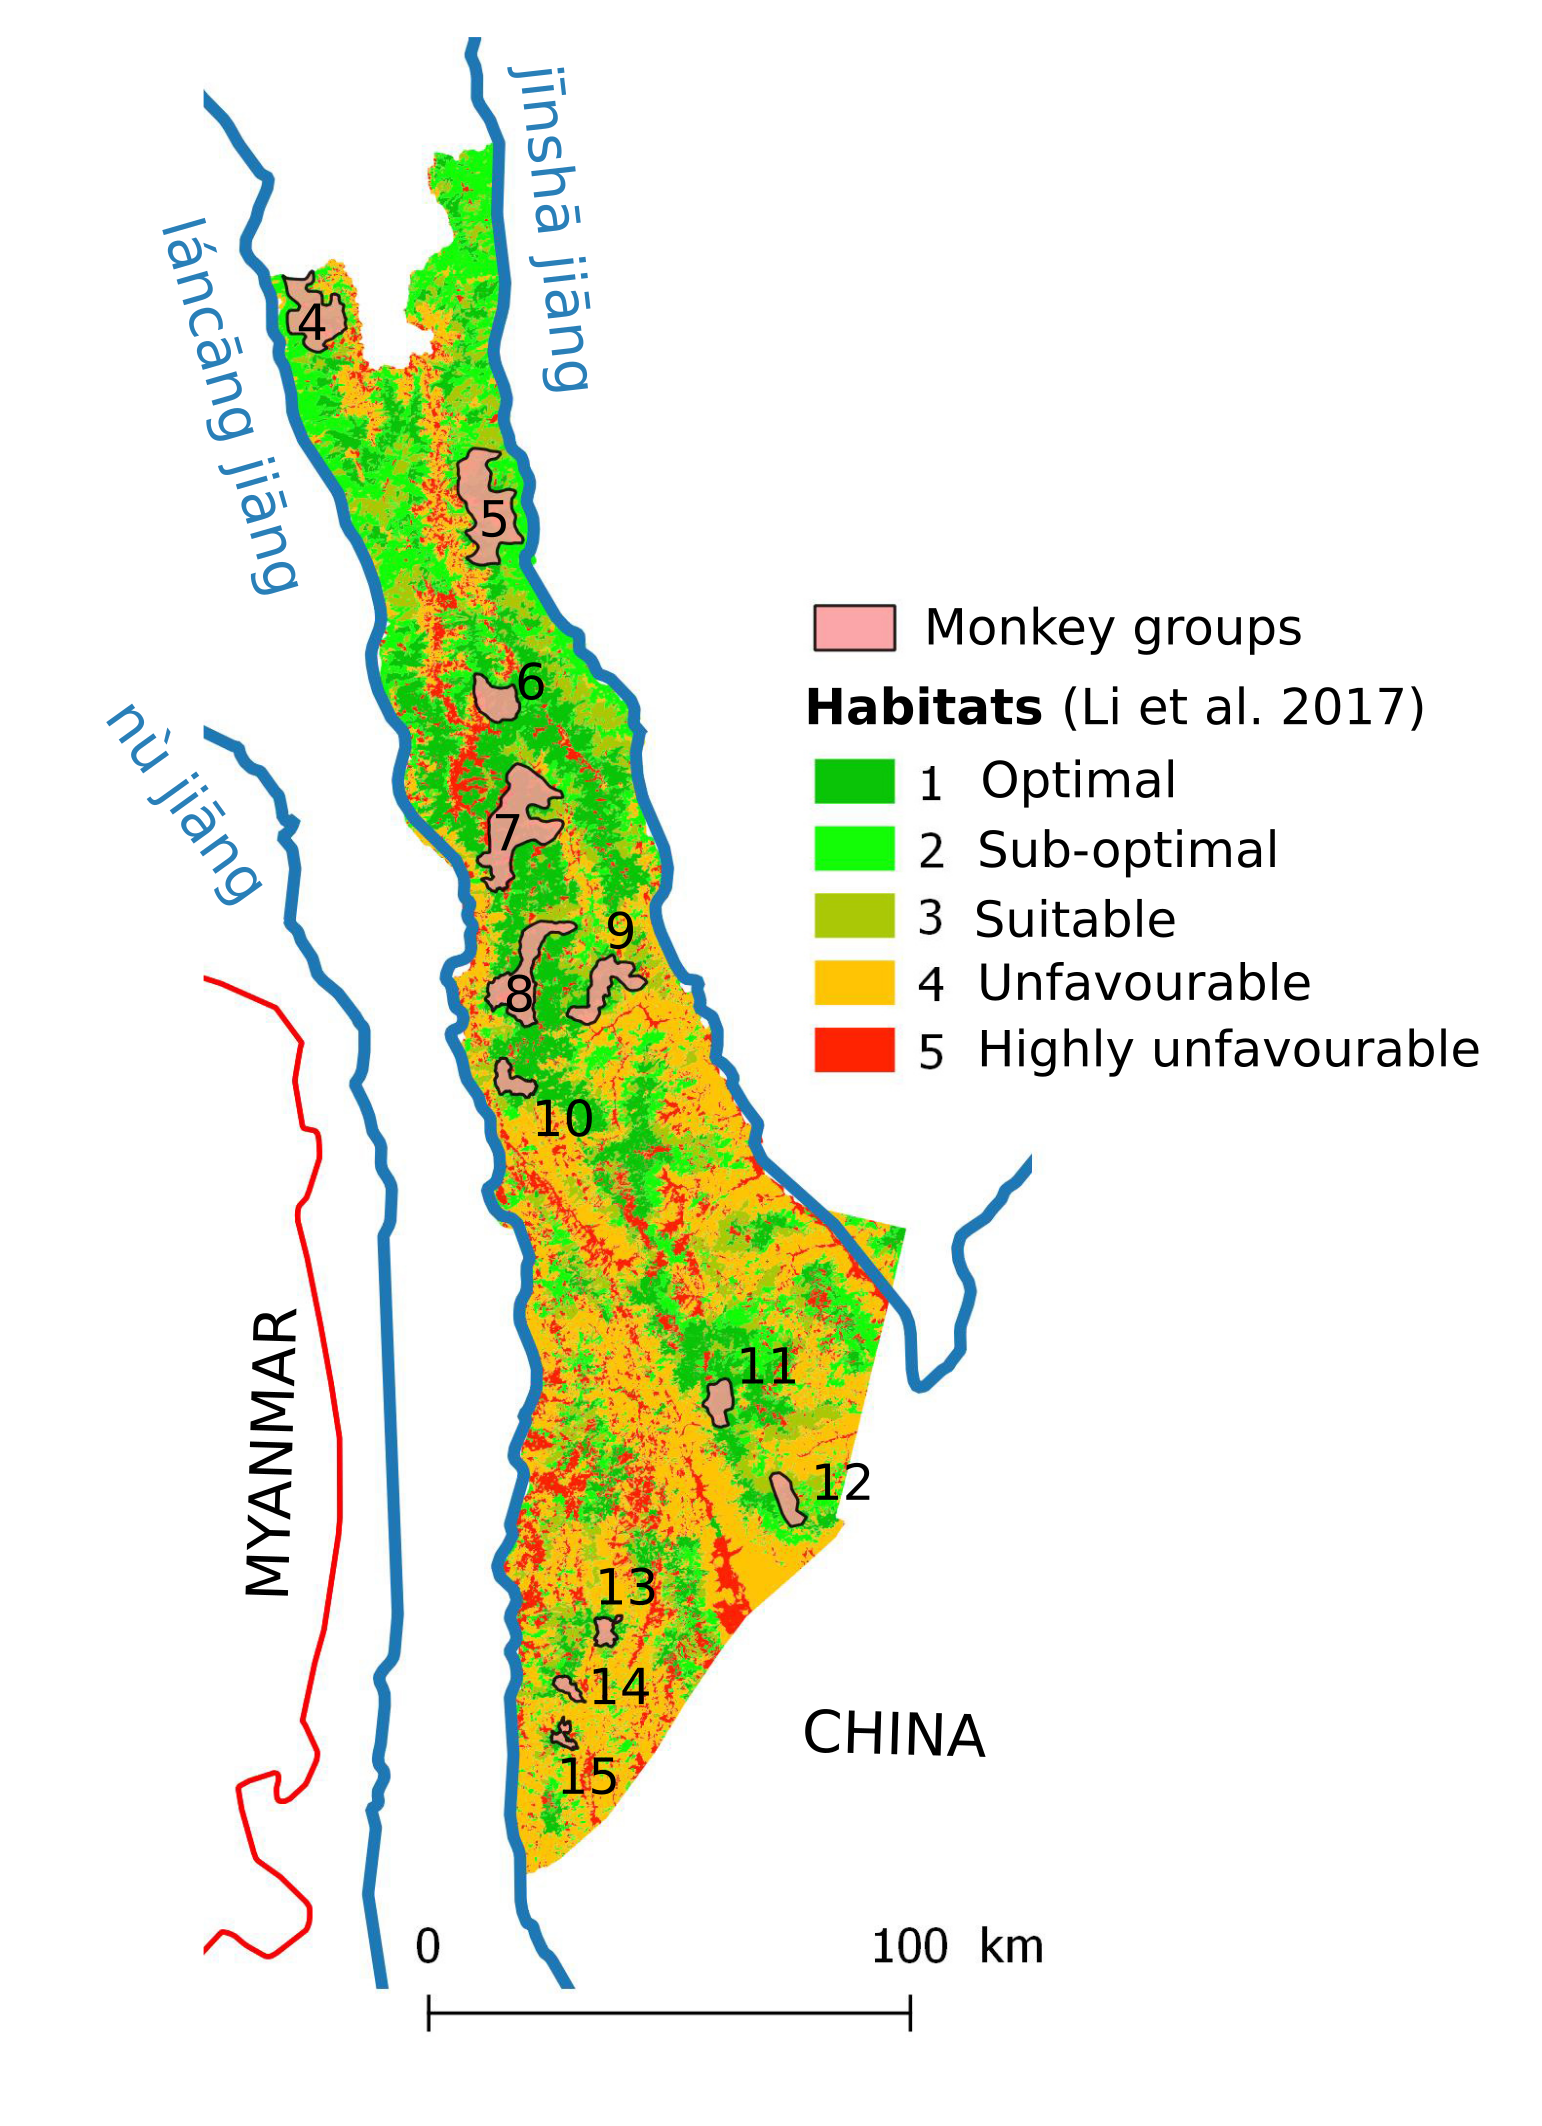
\includegraphics[width=12cm]{Map}
 	\caption{Study area. Numbers on the  map are the group IDs.}
 	\label{fig:studyarea}
 \end{figure}

\section{Model purpose}
Here we want to build a multi-agent model to simulate and explore the effect of habitat and life-history trait 
parameters (real values known or unknown) on snubby dispersion.

\section{Model parameters}

\subsection{Input parameters}
\begin{description}
	\item[step] 1 hour (the iteration time resolution)
	\item[maximum speed] the maximum speed (km/day) that can sustain a snubby in a favourable habitat
	\item[maximum survival]  [0,1] the maximum survival in a favourable habitat. The end user give it per year ($s_y$), but this should be converted to the scale of the step (here hour), using the following formula:
	$s_h=e^{\frac{\ln{s_y}}{365\times24}}$
	\item[disperser proportion] the proportion of snubbies who evade their group and wander outside. The end user give it per year  ($p_y$), but this should be converted to the scale of the step (hour): $p_h=e^{\frac{\ln{p_y}}{365\times24}}$
	\item[habitat viscosity] [0,1] the resistance of a given habitat.  Multiplies the maximum speed to give the speed really sustained in this habitat.
	\item[habitat security] [0,1] the security of a given habitat.  Multiplies the maximum survival to give the actual survival in this habitat.
	\item[habitat dislike] [0,0.5] the probability for a snubby to move into a habitat of lesser quality.
	\item[habitat preference] [0.5,1] the probability for a snubby to move into a habitat of better quality.
	
\end{description}

\subsection{During simulation}
When one snubby dies, one snubby is created in its aboriginal group.


\subsection{Output parameters}

\begin{description}
	\item[Bitmap] Bitmap of snubby distribution (framerate: 6 months).
	\item[Shapefile] Shapefile of snubby distribution with their individual attributes (framerate: 1 year).
	\item[group composition and wanderers] Snubby number in each group and outside, split by group origin.
	
\end{description}





